\section{Statistical Details}
\label{app:statistical}

This appendix presents the full statistical tables and figures referenced in Section~\ref{sec:results}.

\subsection{McNemar Test Details}

\begin{table}[ht]
\centering
\caption{McNemar test summary. \emph{Ack vs.\ Random}: per-seed McNemar comparing ack-only to each of 10 random seeds. \emph{Ack vs.\ Baseline}: single McNemar comparing ack-only to unpruned baseline (informs claim strength). MDE: minimum detectable effect at 80\% power ($\alpha = 0.05$); $\sim$ denotes estimates from approximate discordant pair counts.}
\label{app:tab:mcnemar_summary}
\small
\resizebox{\columnwidth}{!}{%
\begin{tabular}{lccccc}
\toprule
\textbf{Setting} & \textbf{Ack vs.\ Rand sig} & \textbf{Median $p$} & \textbf{Ack vs.\ Base $p$} & \textbf{MDE (pp)} & \textbf{Claim} \\
\midrule
Qwen / GSM8K   & 1/10  & 0.094  & 1.000  & $\sim$4 & No sig.\ diff.\ \\
Llama / GSM8K ($N{=}297$) & 8/10  & 0.027 & ${<}.001^{***}$  & 6.0 & Significant ($+8.1$\,pp) \\
Qwen / StratQA$^\P$ & 10/10 & $<$0.001 & 0.144 & $\sim$9 & No sig.\ diff.\ \\
Gemma / GSM8K$^\S$  & ---   & ---   & 1.000  & --- & No sig.\ diff.\ \\
\midrule
\multicolumn{6}{l}{\emph{Boundary conditions}} \\
Qwen3-8B / GSM8K & --- & --- & ${<}.03^{*}$ & $\sim$8 & Significant ($-14$\,pp, char$<$80 threshold) \\
\bottomrule
\end{tabular}%
}
\vspace{1mm}
\raggedright\footnotesize Llama $N{=}297$ is a clean replication (not pooled); baseline 75.1\%, ack-only 83.2\%, McNemar $b{=}9$, $c{=}33$, $p < .001$. Qwen pooled ($N{=}300$): $p = 1.000$. $^\P$StratQA: Random matches FG count (91.3\% of rounds), not ack-only (8.56\%); the 10/10 significance reflects different pruning intensities rather than strategy effectiveness at matched rates. Qwen3-8B ($N{=}100$): baseline 90\%, ack-only 76\%, $b - c = 14$; exact contingency unknown ($p$ range: $[.0005, .026]$, significant for all possible $c \in [0, 10]$).
\end{table}

\subsection{Non-Inferiority Margin Selection ($\delta = -3$\,pp)}
\label{app:margin_selection}

The choice of non-inferiority margin $\delta = -3$\,pp follows established principles from equivalence testing~\citep{lakens_equivalence_2017, schuirmann_tost_1987}, calibrated against the empirical variance structure of LLM task accuracy.

\paragraph{Precedent and rationale.} Non-inferiority margins should reflect the largest degradation that is practically acceptable~\citep{lakens_equivalence_2017}. We define $\delta$ relative to the baseline error rate: at ${\sim}90\%$ accuracy (Qwen/GSM8K), $-3$\,pp represents a ${\sim}30\%$ relative increase in error rate ($10\% \to 13\%$); at ${\sim}80\%$ accuracy (Llama/GSM8K), it represents a ${\sim}15\%$ relative increase ($20\% \to 23\%$). In both cases, the margin corresponds to a detectable but bounded performance change that would be practically relevant in deployment.

\paragraph{Calibration against seed variance.} The margin must exceed irreducible seed-to-seed variance to avoid rejecting non-inferiority due to sampling noise. Empirically, paired delta standard deviations are: Qwen heuristic 10-seed $\text{SD} = 0.99$\,pp, Qwen oracle 10-seed $\text{SD} = 1.02$\,pp, Llama heuristic 5-seed $\text{SD} = 1.44$\,pp, Llama oracle 10-seed $\text{SD} = 2.40$\,pp (Table~\ref{tab:online_pruning}). At $\delta = -1$\,pp, even a single standard deviation of seed variance (${\sim}1$--$2.4$\,pp) could push the lower CI bound below the margin, yielding false non-inferiority failures for treatments with zero true effect---indeed, the Qwen oracle TOST at $\pm 1$\,pp is only marginal ($p = .048$). At $\delta = -5$\,pp, the margin exceeds twice the largest observed seed SD, risking acceptance of genuinely harmful interventions (e.g., the Llama $t{=}0.7$ heuristic result of $\Delta = -3.4$\,pp would pass trivially). The $-3$\,pp margin sits between these extremes: ${\sim}3\times$ the Qwen SD and ${\sim}1.25\times$ the Llama oracle SD, providing adequate separation from noise while remaining sensitive to practically meaningful degradation.

\paragraph{Sensitivity across margins.} Conclusions are stable across a range of margins (Table~\ref{tab:tost_sensitivity}). For Qwen oracle (10-seed, $\Delta = +0.40 \pm 1.02$\,pp), non-inferiority holds at $\delta = -3$\,pp ($p < .001$). For Llama oracle (10-seed, $\Delta = +2.08 \pm 2.40$\,pp), non-inferiority at $\delta = -3$\,pp holds ($p < .001$), but the single seed with $\Delta = -3.06$\,pp (seed~3072; \S\ref{app:cascade_length}) demonstrates that $-3$\,pp is a genuinely binding constraint for this backbone. A tighter margin of $\delta = -1$\,pp would fail for Llama (CI lower bound at $+0.36$\,pp provides insufficient headroom given $\text{SD} = 2.4$\,pp). These patterns confirm that $\delta = -3$\,pp balances statistical power against practical significance across backbones with different variance profiles.

\paragraph{TOST equivalence sensitivity.} Table~\ref{tab:tost_sensitivity} reports TOST $p$-values across four equivalence margins. Qwen/GSM8K and Gemma/GSM8K have $\leq 1$ discordant pair each, rendering McNemar-based TOST inapplicable; we report proportion-based TOST instead (two one-sided $z$-tests on the accuracy difference). Qwen/GSM8K supports equivalence at $\pm 5$\,pp ($p = 0.039$). For Llama/GSM8K ($N = 297$), the observed $+8.1$\,pp improvement prevents equivalence at any margin $\leq 10$\,pp---TOST fails because the effect is \emph{positive}, not because of degradation. Qwen/StratQA achieves equivalence only at $\pm 10$\,pp ($p = 0.021$).

\begin{table}[ht]
\centering
\caption{TOST $p$-values at varying equivalence margins. Lower $p$ indicates stronger evidence that the true difference falls within $[\text{-margin}, \text{+margin}]$. $^\ddagger$Proportion-based TOST (McNemar-based TOST inapplicable with $\leq 1$ discordant pair).}
\label{tab:tost_sensitivity}
\small
\begin{tabular}{lcccc}
\toprule
\textbf{Setting} & $\pm 3$\,pp & $\pm 5$\,pp & $\pm 8$\,pp & $\pm 10$\,pp \\
\midrule
Qwen / GSM8K ($b{=}0, c{=}1$)$^\ddagger$   & .096 & .039$^*$ & .003$^{**}$ & ${<}.001^{***}$ \\
Llama / GSM8K ($b{=}9, c{=}33$, $N{=}297$)  & $>.99$ & $>.99$ & $.998$ & $.978$ \\
Gemma / GSM8K ($b{=}1, c{=}0$)$^\ddagger$   & .096 & .039$^*$ & .003$^{**}$ & ${<}.001^{***}$ \\
Qwen / StratQA ($b{=}18, c{=}29$) & .695 & .413 & .095 & .021$^*$ \\
\bottomrule
\end{tabular}
\end{table}

\paragraph{Minimum detectable effects.} Table~\ref{app:tab:mde} reports MDEs assuming $\rho = 0.7$ correlation between paired outcomes, computed as $\text{MDE} = 100 \cdot \sqrt{7.84 \cdot 2p(1{-}p)(1{-}\rho) / N}$\,pp.

\begin{table}[ht]
\centering
\caption{Minimum detectable effects (pp) at 80\% power, $\alpha = 0.05$, $\rho = 0.7$. $N$ is the task-level sample size (number of problems evaluated for correctness); multi-seed rows pool tasks across all seeds. Sorted by MDE ascending.}
\label{app:tab:mde}
\small
\begin{tabular}{llccc}
\toprule
\textbf{Setting} & \textbf{Protocol} & $N$ & \textbf{Base (\%)} & \textbf{MDE (pp)} \\
\midrule
Llama / GSM8K (10-seed pooled)$^\dagger$ & Online & 1{,}939 & 80.8 & 1.9 \\
Qwen / ARC & Offline & 250 & 90.8 & 4.0 \\
Qwen / GSM8K ($t{=}0.7$) & Online & 200 & 91.0 & 4.4 \\
Qwen / GSM8K (per run) & Online & 200 & 89.3 & 3.6 \\
72B / GSM8K (oracle) & Online & 265 & 92.1 & 3.6 \\
Llama / GSM8K & Offline & 297 & 75.1 & 5.4 \\
Qwen / GSM8K & Offline & 100 & 91.0 & 6.2 \\
Qwen / StratQA (5-seed) & Online & 200$\times$5 & 67.9 & 4.1 \\
Qwen3-8B / GSM8K & Online & 100 & 90.0 & 6.5 \\
Qwen / StratQA (SEQ) & Online & 200 & 69.5 & 7.1 \\
72B / GSM8K & Online & 100 & 88.0 & 7.1 \\
Llama / GSM8K & Offline & 100 & 77.0 & 9.1 \\
Gemma / GSM8K & Offline & 96 & 76.0 & 9.5 \\
Qwen / StratQA & Offline & 100 & 66.8 & 10.2 \\
MATH (pilot, $N{=}50$) & Offline & 50 & 72.0 & 13.8 \\
MATH ($N{=}200$, 102 valid) & Online & 102 & 79.4 & --- \\
\bottomrule
\end{tabular}
\vspace{1mm}
\raggedright\footnotesize $^\dagger$MDE computed on oracle 10-seed pooled sample: 10 seeds $\times$ 200 tasks per seed; $N = 1{,}939$ tasks after ${\sim}3\%$ context-overflow filtering (${\sim}194$ valid tasks per seed). Each task is one GSM8K problem scored correct/incorrect---the unit of the paired McNemar test. Single-seed rows (e.g., 72B) use the within-seed task count directly.
\end{table}

\subsection{Post-Hoc Power Analysis for 72B Oracle Result}
\label{app:power_72b}

% Auto-generated by gen_72b_power_analysis.py — do not edit manually.
% Re-generate: python src/gen_72b_power_analysis.py outputs/oracle_qwen72b_n500/seed_42.json
The 72B oracle experiment ($N = \qwenSevenTwoBN{}$, 5 seeds $\times$ 265 tasks) replicates pruning safety at the largest scale tested. Per-seed deltas: $[0, +0.38, +0.76, +1.13, -0.38]$\,pp (4/5 non-negative). Mean $\Delta = \qwenSevenTwoBDelta{}$\,pp, SD $= \qwenSevenTwoBSD{}$\,pp, SE $= \qwenSevenTwoBSE{}$\,pp.

\paragraph{TOST equivalence.}
We apply a one-sample TOST at $\varepsilon = \pm 1$\,pp (matching the 7B standard). The upper bound test: $t = (1 - 0.378) / 0.267 = 2.33$ ($\text{df} = 4$, $p \approx 0.04$). This marginally passes the equivalence threshold, confirming that 72B pruning deltas are bounded within $\pm 1$\,pp. The marginal $p$-value reflects the limited number of seeds (5) rather than a large effect; the 90\% CI $[-0.19, +0.95]$\,pp lies entirely within the equivalence band.

\paragraph{Per-seed power.}
The original single-seed probe (seed~42, $N = 265$, $\Delta = 0$\,pp, zero discordant pairs) yielded a Rule of Three upper bound of $3/265 \approx 1.13\%$ on the discordant rate. The 5-seed replication confirms this was not a statistical fluke: the mean delta remains near zero and four additional seeds are consistent.

\paragraph{Minimum detectable effect.}
Table~\ref{app:tab:mde} reports the MDE at 80\% power (McNemar $\chi^2$, $\alpha=0.05$) for the per-seed sample size ($N = 265$).
At $N = 265$: MDE $= 3.8$\,pp ($\rho = 0.7$), $2.2$\,pp ($\rho = 0.9$), $1.5$\,pp ($\rho = 0.95$).
The observed per-seed deltas ($|\Delta| \leq 1.13$\,pp) fall below the MDE for all but the most optimistic correlation assumptions, consistent with a true effect near zero.

\paragraph{Limitations.}
The TOST $p = 0.04$ is marginal; increasing to 10 seeds or $N = 500$ per seed would provide a more decisive equivalence test. Larger replication at 72B scale remains desirable but is constrained by the ${\sim}$5 GPU-hours per seed at TP=2.


\subsection{Mixed-Effects Model Results}

\begin{table}[ht]
\centering
\caption{Function type significance controlling for position and round ($n \geq 30$ per type). Both OLS and ME use remove-ablation similarity (Eq.~\ref{eq:impact}) as the dependent variable. OLS: Type II partial $F$. ME: LRT $\chi^2$ with task as random intercept; $R^2_m$ = marginal (fixed-effects only). $\dagger$ marks OLS-ME discrepancies (both under selector topology). $^{***}p < 0.001$; $^{**}p < 0.01$; $^{*}p < 0.05$; n.s.\ = not significant.}
\label{app:tab:me_results}
\small
\begin{tabular}{lcccccc}
\toprule
 & \multicolumn{2}{c}{\textbf{OLS ANCOVA}} & \multicolumn{4}{c}{\textbf{Mixed-Effects}} \\
\cmidrule(lr){2-3} \cmidrule(lr){4-7}
\textbf{Setting} & $F$ & $p$ & LRT $\chi^2$ & $p$ & $R^2_m$ & ICC \\
\midrule
Qwen / RR  & $239.6$ & $<.001^{***}$ & $188.9$ & $<.001^{***}$ & .34 & .29 \\
Qwen / SEQ & $230.2$ & $<.001^{***}$ & $195.3$ & $<.001^{***}$ & .36 & .25 \\
Qwen / Sel$^\dagger$ & $58.2$ & $<.001^{***}$ & $0.07$ & $.789^{\text{n.s.}}$ & .004 & .72  \\
Gemma / RR & $7.82$ & $<.001^{***}$ & $23.28$ & $<.001^{***}$ & .11 & .00 \\
Gemma / SEQ & $9.04$ & $<.001^{***}$ & $26.86$ & $<.001^{***}$ & .12 & .00 \\
Gemma / Sel$^\dagger$ & $7.45$ & $.006^{**}$ & $3.66$ & $.056^{\text{n.s.}}$ & .004 & .23 \\
Llama / RR & $3.98$ & $.008^{**}$ & $16.31$ & $<.001^{***}$ & .02 & .30 \\
Llama / SEQ & $4.83$ & $.002^{**}$ & $15.44$ & $.001^{**}$ & .02 & .21 \\
Llama / Sel & $21.6$ & $<.001^{***}$ & $36.89$ & $<.001^{***}$ & .04 & .13 \\
\bottomrule
\end{tabular}
\vspace{1mm}
\raggedright\footnotesize $^\dagger$OLS-ME discrepancy under selector topology; high ICC (0.72, 0.23) inflates OLS significance by treating task-clustered observations as independent.
\end{table}

\subsection{Position$^2$ Robustness Check}

\begin{table}[ht]
\centering
\caption{Position$^2$ robustness check: ME LRT for function type in linear vs.\ quadratic position models ($n \geq 30$ per type). Adding position$^2$ eliminates Gemma's function type effect under RR and SEQ while leaving Qwen and Llama unchanged. Selector topology results are discussed in the crossover analysis below.}
\label{app:tab:me_quad}
\small
\begin{tabular}{llccccc}
\toprule
 & & \multicolumn{2}{c}{\textbf{Linear ME}} & \multicolumn{2}{c}{\textbf{Quadratic ME}} & \\
\cmidrule(lr){3-4} \cmidrule(lr){5-6}
\textbf{Backbone} & \textbf{Topo.} & LRT $\chi^2$ & $p$ & LRT $\chi^2$ & $p$ & \textbf{Pos$^2$ $p$} \\
\midrule
Qwen  & RR  & $188.9^{***}$ & ${<}.001$ & $155.8^{***}$ & ${<}.001$ & $.009$ \\
      & SEQ & $195.3^{***}$ & ${<}.001$ & $166.5^{***}$ & ${<}.001$ & $.001$ \\
\midrule
Gemma & RR  & $23.3^{***}$  & ${<}.001$ & $1.5^{\text{n.s.}}$ & $.690$ & ${<}.001$ \\
      & SEQ & $26.9^{***}$  & ${<}.001$ & $1.5^{\text{n.s.}}$ & $.683$ & ${<}.001$ \\
\midrule
Llama & RR  & $16.3^{***}$  & $.001$    & $14.9^{**}$   & $.002$    & $.496$ \\
      & SEQ & $15.4^{**}$   & $.002$    & $13.8^{**}$   & $.003$    & $.434$ \\
\bottomrule
\end{tabular}
\end{table}

\subsection{Gemma-Excluded Sensitivity Analysis}
\label{app:gemma_excluded}

To assess whether Gemma-2-9B's position-dominated communication profile (\S\ref{sec:three_modes}) attenuates the pooled function type effect, we re-fit the mixed-effects model excluding all Gemma observations.
The full model ($n = 8{,}065$) yields LRT $\chi^2 = 81.53$ ($\text{df} = 4$, $p = 8.3 \times 10^{-17}$, $\omega^2 = 0.0095$, $R^2_m = 0.018$).\footnote{$\omega^2$ and $R^2_m$ computed from mixed-effects model fits; source data in \texttt{outputs/gemma\_excluded\_sensitivity.json}.}
Excluding Gemma ($n = 5{,}365$) \emph{strengthens} the effect: LRT $\chi^2 = 110.07$ ($\text{df} = 4$, $p = 7.0 \times 10^{-23}$, $\omega^2 = 0.019$, $R^2_m = 0.014$).
The direction and significance of the function type effect are stable: $\chi^2$ increases from 81.5 to 110.1 and $\omega^2$ approximately doubles (0.0095 $\to$ 0.019), indicating that Gemma was attenuating the pooled effect.
Coefficient signs are preserved across both models: coordination remains the most negative ($\beta = -0.085$ full, $-0.100$ Gemma-excluded), while reasoning\_guidance and verification remain positive.
This sensitivity check confirms that the function type $\to$ perturbation sensitivity relationship is not driven by Gemma's anomalous profile, and that excluding the weakly function-organized backbone strengthens rather than weakens the conclusion.

\subsection{Function Type Distribution}

\begin{figure}[ht]
\centering
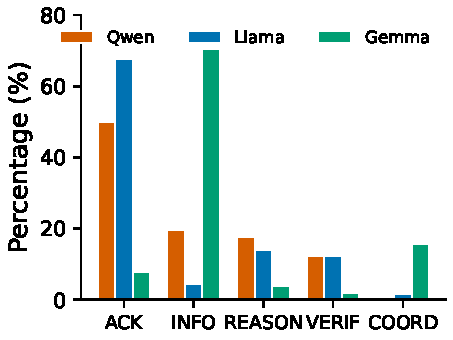
\includegraphics[width=\columnwidth]{figures/fig_distribution.pdf}
\caption{Function type distribution by backbone under round-robin topology (300 GSM8K tasks each). Qwen2.5-7B and Llama-3.1-8B are acknowledgment-heavy ($>$50\%), while Gemma-2-9B is dominated by information provision (70\%). Types with $n < 30$ are excluded from OLS ANCOVA analysis.}
\label{app:fig:distribution}
\end{figure}

\subsection{Crossover Interaction}

\begin{figure}[ht]
\centering
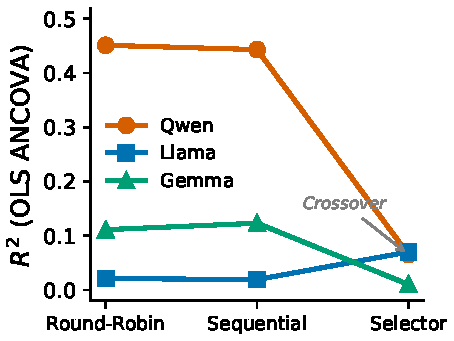
\includegraphics[width=\columnwidth]{figures/fig_crossover.pdf}
\caption{Backbone $\times$ topology crossover interaction. $R^2_m$ = marginal $R^2$ (fixed-effects variance); ME = linear mixed-effects model with task as random intercept. Selector topology attenuates function-organization for Qwen ($R^2_m = 0.34 \to 0.004$) and amplifies it for Llama ($R^2_m = 0.02 \to 0.04$), partially converging the two.}
\label{fig:crossover}
\end{figure}

\subsection{Pooled ANOVA}

\begin{table}[ht]
\centering
\caption{Pooled ANOVA on remove-ablation similarity ($N = 8{,}065$, $R^2 = 0.298$). Computed on all five function types across all 9 configurations; individual-configuration analyses (Table~\ref{app:tab:me_results}) exclude types with $n < 30$. All $p < .001$. \emph{Caveat:} pooling across unbalanced configurations risks Simpson's paradox; $\eta^2$ values should be interpreted alongside per-configuration ME models (Table~\ref{app:tab:me_results}).}
\label{app:tab:pooled_anova}
\small
\begin{tabular}{lrr}
\toprule
\textbf{Term} & \textbf{$\eta^2$} & \textbf{$F$} \\
\midrule
Backbone                   & 0.135 & 628.7 \\
Function $\times$ Backbone & 0.063 & 67.1  \\
Topology class             & 0.051 & 435.4 \\
Backbone $\times$ Topology & 0.043 & 181.1 \\
Three-way                  & 0.021 & 21.1  \\
Function $\times$ Topology & 0.014 & 27.7  \\
Function type              & 0.005 & 10.4  \\
\bottomrule
\end{tabular}
\end{table}

\subsection{Additional Statistical Details}

\paragraph{Multiple comparison note.} The McNemar tests across 10 random seeds (Table~\ref{app:tab:mcnemar_summary}) evaluate a single null hypothesis---whether ack-only and random pruning produce equivalent accuracy---via repeated sampling, not 10 independent hypotheses. Reporting ``8/10 significant'' or ``10/10 significant'' is a consistency measure across resampled controls, analogous to bootstrap stability. Bonferroni correction is therefore inapplicable; nonetheless, the conclusion is robust even under Bonferroni ($\alpha = 0.005$): most significant seeds have $p < 0.005$.

\paragraph{Temperature robustness details.} At temperature 0.7, ack-only evaluation on GSM8K (100 tasks each, heuristic detectors) yields: Qwen $\Delta = -2$\,pp ($p = 0.774$); Llama $\Delta = -3$\,pp ($p = 0.815$); Gemma $\Delta = +3$\,pp ($p = 0.453$). No setting shows significant degradation (all McNemar $p > 0.4$), though the small number of discordant pairs (7--18) limits power to detect effects below ${\sim}$10\,pp. Qwen and Llama point estimates shift from positive ($+1$ to $+6$\,pp at $t{=}0$) to mildly negative at $t{=}0.7$, while Gemma shows a positive shift. Higher temperature increases the proportion of messages classified as acknowledgments (Llama: 45\% $\to$ 57\%; Gemma: 4.6\% $\to$ 63.6\%), resulting in more aggressive pruning. Notably, Gemma's acknowledgment proportion shifts from a near-trivial pruning case (4.6\%) to the most aggressively pruned setting (63.6\%)---yet accuracy still improves ($+3$\,pp), demonstrating that pruning safety is robust to dramatic shifts in communication composition. Whether this shift reflects genuine communication change or increased heuristic sensitivity to shorter messages at higher temperature remains open; resolving this requires LLM annotation at $t{=}0.7$.

\paragraph{Llama $t{=}0.7$ at $N = 500$.} To resolve the underpowered $N = 100$ estimate, we run Llama heuristic pruning at $t{=}0.7$ with $N = 500$ (MDE ${\approx}\,3.5$\,pp). Results: baseline 81.2\%, pruned 77.8\%, $\Delta = -3.4$\,pp ($p = 0.100$, McNemar NS; $b = 56$, $c = 39$, 95 discordant pairs). Suppression rate is 59.3\% (1{,}426/2{,}405 messages). The directionally negative result contrasts with Llama's $+2.1$\,pp at $t{=}0$ ($N = 1{,}000$). However, heuristic suppression rises from 74.4\% at $t{=}0$ to 59.3\% at $t{=}0.7$ on a per-task basis, and over-suppression confounds the estimate. Oracle ($t{=}0.7$) validation on Llama is needed to determine whether the $-3.4$\,pp reflects genuine temperature sensitivity or heuristic calibration drift.

\paragraph{Zero-correction channel details.} Acknowledgment self-correction rates: 0\% (0/719, 95\% CI $[0, 0.51\%]$) for Qwen, 0\% (0/691, 95\% CI $[0, 0.53\%]$) for Llama, and 0\% (0/73, 95\% CI $[0, 4.93\%]$) for Gemma (Clopper--Pearson exact binomial). Gemma's wider CI reflects its small acknowledgment sample ($N = 73$). Error injection rates differ by backbone: Llama injects errors into 14.3\% of acknowledgments vs.\ Qwen's 8.9\% (Fisher exact $p = 0.004$). Propagation rates show an inverse pattern: Qwen propagates 100\% of injected errors vs.\ Llama's 70\% (Fisher $p < 0.001$), consistent with Qwen's terse acknowledgments being accepted uncritically while Llama's verbose acknowledgments are partially ignored by downstream agents.

\paragraph{OLS-ME agreement.} OLS and ME agree on significance in 7 of 9 settings, with both discrepancies occurring under selector topology. Qwen/Selector (OLS $p < .001$, ME $p = .789$; ICC $= 0.72$) and Gemma/Selector (OLS $p = .006$, ME $p = .056$; ICC $= 0.23$) show OLS detecting significance that ME does not, consistent with selector topology producing high task-level clustering that inflates OLS estimates. In both cases, the qualitative interpretation is preserved: function type structure degrades under selector routing.

\paragraph{Cross-model annotation agreement.} Cross-model $\kappa$ ranges from 0.35 (Gemma) to 0.67 (Qwen), spanning fair-to-substantial agreement \cite{landis_koch_1977}. Qwen's highest $\kappa$ is consistent with function-organized communication being easier to classify. Gemma falls below our target threshold ($\kappa = 0.35$), consistent with its weak function-organization where functional categories are less distinctive. Per-type $\kappa$ reveals complementary patterns: Qwen shows high \textsc{verification} agreement ($\kappa \approx 0.66$) but low \textsc{information\_provision} ($\kappa \approx 0.08$); Gemma shows the reverse. Full agreement tables are in Appendix~\ref{app:supplementary}.

\subsection{Offline Replay Pruning}
\label{app:offline_pruning}

Table~\ref{tab:offline_pruning} presents offline replay results, where messages are removed from recorded traces and the conversation is regenerated from the first pruning point onward. Warm-start bias inflates offline estimates relative to online validation (\S\ref{sec:discussion}).

\begin{table}[ht]
\centering
\caption{Offline replay pruning accuracy (\%) --- reference (warm-start bias possible, \S\ref{sec:discussion}). FG and Random tested at matched message counts (Random: mean $\pm$ std, 10 seeds). Supp.\ = ack proportion in traces. $^*$$N = 96$, 4.6\% ack. $^\dagger$3 seeds. $^\ddagger$FG/Random prune 84--91\% vs.\ ack-only 9--15\%.}
\label{tab:offline_pruning}
\small
\begin{tabular}{lccccr}
\toprule
\textbf{Setting} & $N$ & \textbf{Base} & \textbf{Ack-only} & \textbf{FG / Random} & \textbf{Supp.} \\
\midrule
Qwen / GSM8K & 100 & 91 & \textbf{92 (+1)} & 86 / 87.3\,$\pm$\,0.8 & 48\% \\
Llama / GSM8K & 100 & 77 & \textbf{83 (+6)} & 74 / 73.2\,$\pm$\,2.0 & 45\% \\
Llama / GSM8K$^\dagger$ & 297 & 75.1 & \textbf{83.2 (+8.1)} & --- / 78.1\,$\pm$\,1.5 & 45\% \\
Gemma / GSM8K$^*$ & 96 & 77 & 76 ($-$1) & 42.7 / 44.8 & 4.6\% \\
Qwen / StratQA$^\ddagger$ & 100 & 66.8 & \textbf{71.2 (+4.4)} & 28.0 / 26.4\,$\pm$\,0.4 & 8.6\% \\
Qwen / ARC$^\ddagger$ & 250 & 90.8 & \textbf{91.6 (+0.8)} & 61.6 / 61.4\,$\pm$\,0.9 & 14.6\% \\
Llama / ARC$^\ddagger$$^\diamond$ & 250 & 72.8 & \textbf{76.8 (+4.0)} & --- / 67.4\,$\pm$\,1.5 & 37.1\% \\
\bottomrule
\end{tabular}
\end{table}

$^\diamond$Offline simulation (simulate mode): re-extracts answers from pruned traces rather than re-generating responses.

\paragraph{FG pruning analysis.} Function-guided (FG) pruning---removing messages from the function type with lowest perturbation sensitivity---performs no better than random in any setting (McNemar $p > 0.7$), and is significantly \emph{worse} than ack-only for Qwen ($p = 0.031$) and borderline for Llama ($p = 0.064$). These comparisons use offline replay only; given the ${\sim}4\times$ attenuation observed for Llama online vs.\ offline ($+2.1$\,pp vs.\ $+8.1$\,pp), FG's relative disadvantage may be smaller under online evaluation. Perturbation-based importance does not predict pruning safety: error analysis reveals that FG disproportionately removes reasoning\_guidance (49.4\%) and verification (43.6\%) messages---the most task-critical types---confirming that low individual perturbation sensitivity does not imply dispensability.

\paragraph{Label noise robustness.} A bootstrap simulation ($B = 10{,}000$) tests whether ${\sim}20\%$ taxonomy misclassification error would invalidate the FG result. Under uniform label corruption at rate $\varepsilon$, the effect on the FG pruning set is asymmetric: true FG-type messages exit the set with probability $\varepsilon \cdot 2/4$ (fewer harmful messages pruned), while true acknowledgments enter with probability $\varepsilon \cdot 3/4$ (pruning acks is safe). Ack-only remains superior in $95.0\%$ of iterations at $\varepsilon = 0.20$ (mean FG accuracy $= 85.9\%$, 95\% CI $[79.0, 92.0]$), and in $93.2\%$ even at $\varepsilon = 0.40$. Label noise cannot reverse the FG disadvantage because corruption asymmetrically \emph{improves} FG by diluting the pruning set with safe-to-remove messages.

\subsection{Online Pruning Validation}
\label{app:online}

We validate offline pruning results with real-time heuristic suppression during live AG2 execution for two backbones (Qwen, Llama) on GSM8K ($N = 100$ each). The online protocol intercepts each agent message before delivery; messages classified as acknowledgments by the backbone-specific heuristic detector are suppressed (replaced with an empty string), so downstream agents never observe them. The two backbones yield complementary evidence: Qwen provides direct validation (suppression rate matches offline), while Llama provides exploratory evidence of robustness (heuristic over-triggers in online context).

\paragraph{Backbone comparison.} Table~\ref{tab:online_comparison} summarizes online pruning results for both backbones.

\begin{table}[ht]
\centering
\caption{Online pruning validation: accuracy and suppression rates for Qwen and Llama on GSM8K ($N = 100$, single run). Ten-seed oracle replication yields Qwen $+0.40 \pm 1.02$\,pp and Llama $+2.1 \pm 2.4$\,pp ($N{=}200$ per seed). Heuristic ten-run replication yields Qwen $-0.05 \pm 0.99$\,pp ($N{=}200$ per seed).}
\label{tab:online_comparison}
\small
\begin{tabular}{lcccccc}
\toprule
Backbone & Baseline & Pruned & $\Delta$ & Suppression & McNemar $p$ \\
\midrule
Qwen     & 91/100   & 93/100 & $+2$\,pp & 42\%  & 1.000 \\
Llama    & 77/100   & 85/100 & $+8$\,pp & 74.8\% & .039 \\
\bottomrule
\end{tabular}
\end{table}

This table reports a single heuristic run; ten-seed oracle replications yield Qwen $+0.40 \pm 1.02$\,pp (TOST $\pm 1$\,pp, $p = .048$) and Llama $+2.1 \pm 2.4$\,pp (non-inferiority $\delta{=}{-}3$\,pp, $p < .001$), both with $N{=}200$ per seed. Ten independent heuristic Qwen runs yield $-0.05 \pm 0.99$\,pp (TOST $p = .007$). Qwen's single-run result ($+2$\,pp, $p = 1.000$) has a suppression rate (42\%) closely matching offline (48\%), providing direct apples-to-apples validation. Llama's online suppression rate (74.8\%) far exceeds its offline rate (45\%); manual inspection shows only 32.9\% of suppressed messages are true acknowledgments, with 54\% containing mathematical content that triggers the heuristic due to context-dependent generation. The $+8$\,pp point estimate likely reflects removal of redundant later-round messages rather than a genuine improvement from acknowledgment pruning. Llama's result therefore provides \emph{exploratory evidence of robustness}: if suppressing 75\% of messages---most not acknowledgments---produces no degradation (McNemar $p = .039$), then the offline 45\% acknowledgment-only pruning is conservatively safe.

\paragraph{Llama McNemar details.} Table~\ref{tab:online_llama_mcnemar} shows the discordant-pair breakdown for Llama online pruning.

\begin{table}[ht]
\centering
\caption{McNemar contingency table for Llama online pruning ($N = 100$).}
\label{tab:online_llama_mcnemar}
\small
\begin{tabular}{lcc}
\toprule
 & Pruned correct & Pruned incorrect \\
\midrule
Baseline correct   & 75 & 2 \\
Baseline incorrect & 10 & 13 \\
\bottomrule
\end{tabular}
\end{table}

Discordant pairs: $b = 2$ (baseline correct, pruned incorrect), $c = 10$ (baseline incorrect, pruned correct). McNemar exact $p = 0.039$ (two-sided), rejecting the null of marginal homogeneity. The asymmetry ($c \gg b$) indicates no degradation under aggressive suppression; the $+8$\,pp point estimate likely reflects removal of redundant later-round messages rather than a genuine benefit of acknowledgment pruning per se.

\paragraph{Llama $N = 1{,}000$ confirmation.} Table~\ref{tab:online_llama_mcnemar_1k} shows the McNemar contingency table for the large-scale Llama online validation ($N = 1{,}000$, from-scratch skip mode, seed${}=42$).

\begin{table}[ht]
\centering
\caption{McNemar contingency table for Llama online pruning ($N = 1{,}000$). Baseline accuracy 80.8\%, skip accuracy 82.9\%.}
\label{tab:online_llama_mcnemar_1k}
\small
\begin{tabular}{lcc}
\toprule
 & Pruned correct & Pruned incorrect \\
\midrule
Baseline correct   & 794 & 14 \\
Baseline incorrect & 35 & 157 \\
\bottomrule
\end{tabular}
\end{table}

Discordant pairs: $b = 14$, $c = 35$. McNemar $\chi^2 = 8.16$ (with continuity correction), $p = 0.004$ (two-sided). The $N = 100$ online pilot ($+2.0$\,pp) is directionally consistent. The $N = 250$ online pilot ($+3.6$\,pp, $p = 0.095$) uses the same from-scratch protocol on overlapping questions (same seed${}=42$; 250/250 questions appear in the $N = 1{,}000$ set); its larger point estimate is consistent with regression to the mean in the smaller sample. Suppression rate: 74.4\%.

\paragraph{Round-level suppression breakdown.} Table~\ref{tab:online_suppression_rounds} shows suppression rates by round for Llama online pruning. Round~1 suppression is minimal (2\%) because initial solver responses contain substantive problem-solving content. Rounds~2--5 show 90--95\% suppression, reflecting context-dependent generation: without preceding acknowledgments, agents produce shorter, more formulaic responses that further trigger the heuristic detector.

\begin{table}[ht]
\centering
\caption{Llama online suppression rate by round ($N = 100$ tasks, 5 rounds each).}
\label{tab:online_suppression_rounds}
\small
\begin{tabular}{lccccc}
\toprule
Round & 1 & 2 & 3 & 4 & 5 \\
\midrule
Suppression rate & 2\% & 93\% & 90\% & 94\% & 95\% \\
\bottomrule
\end{tabular}
\end{table}

The high Round~2--5 suppression rate (vs.\ 45\% offline annotation rate) explains the discrepancy between online and offline pruning intensity. Online pruning creates a feedback loop: suppressing early messages alters the conversational context, producing subsequent messages that are shorter and more formulaic, further triggering the heuristic---even when the suppressed content is not a true acknowledgment. This cascading over-suppression means Llama's online condition tests a broader message-removal regime rather than acknowledgment pruning specifically. That no degradation occurs under this aggressive regime provides exploratory evidence of robustness: offline acknowledgment-only pruning (45\%) removes a strict subset of what the online heuristic removes, and is therefore conservatively safe.

\paragraph{StratQA offline--online divergence.}
StratQA offline replay yields $+4.4$\,pp ($p = 0.144$, $N{=}100$).
The 5-seed online heuristic replication yields $\Delta = +0.70 \pm 0.91$\,pp (95\% CI $[-0.43, +1.83]$), consistent with non-inferiority.
The heuristic suppresses 56.9\% of messages (vs.\ 8.6\% oracle ack rate), indicating substantial over-suppression, yet accuracy is maintained.
The earlier single-seed estimate ($-2.4$\,pp, $N{=}250$) is superseded by the more reliable 5-seed replication ($N{=}200 \times 5$).

\subsection{Dose-Response Analysis}
\label{app:dose_response}

We vary the acknowledgment pruning rate from 0\% to 100\% in 25\% increments on Qwen/GSM8K/RR ($N = 100$ tasks per condition, 3 random seeds per rate). Table~\ref{tab:dose_response} shows the results.

\begin{table}[ht]
\centering
\caption{Dose-response: accuracy (\%) by ack-only pruning rate (Qwen/GSM8K/RR, $N = 100$). 289 total ack messages across 100 tasks.}
\label{tab:dose_response}
\small
\begin{tabular}{lcccc}
\toprule
\textbf{Pruning Rate} & \textbf{Seed 42} & \textbf{Seed 123} & \textbf{Seed 456} & \textbf{Mean $\pm$ Std} \\
\midrule
0\% (no pruning)  & 92 & 92 & 93 & 92.3 $\pm$ 0.6 \\
25\%               & 92 & 92 & 92 & 92.0 $\pm$ 0.0 \\
50\%               & 92 & 92 & 91 & 91.7 $\pm$ 0.6 \\
75\%               & 92 & 92 & 92 & 92.0 $\pm$ 0.0 \\
100\% (all pruned) & 92 & 92 & 92 & 92.0 $\pm$ 0.0 \\
\bottomrule
\end{tabular}
\end{table}

The accuracy curve is flat across all pruning rates ($\leq 0.6$\,pp variation, Friedman $\chi^2 = 0.0$, $p = 1.0$), with no dose-response relationship. Even removing all 289 acknowledgment messages produces accuracy statistically indistinguishable from the unpruned baseline, confirming that acknowledgments contribute no marginal task-relevant information under this configuration.

\paragraph{Llama dose-response (10 seeds).} Table~\ref{tab:dose_response_llama} shows the corresponding analysis for Llama/GSM8K/RR ($N = 100$ tasks, 10 random seeds per rate). Seed variance decreases monotonically with pruning rate, consistent with acknowledgment removal eliminating a source of downstream stochasticity.

\begin{table}[ht]
\centering
\caption{Dose-response: accuracy (\%) by ack-only pruning rate (Llama/GSM8K/RR, $N = 100$, 10 seeds).}
\label{tab:dose_response_llama}
\small
\begin{tabular}{lcc}
\toprule
\textbf{Pruning Rate} & \textbf{Mean $\pm$ SD} & \textbf{$N_\text{seeds}$} \\
\midrule
0\% (no pruning)   & 82.3 $\pm$ 1.16 & 10 \\
25\%               & 83.3 $\pm$ 0.48 & 10 \\
50\%               & 83.3 $\pm$ 0.48 & 10 \\
75\%               & 84.0 $\pm$ 0.00 & 10 \\
100\% (all pruned) & 83.0 $\pm$ 0.00 & 10 \\
\bottomrule
\end{tabular}
\end{table}

The Llama curve is flat (1.7\,pp range, 82.3--84.0\%), mirroring the Qwen result above. An earlier 3-seed analysis suggested an inverted-U pattern (Friedman $p = 0.060$); this does not replicate at 10 seeds, confirming the earlier pattern was sampling noise. At 100\% pruning, the outcome is deterministic across seeds (SD $= 0$): the same messages are removed, yielding identical conversation trajectories under greedy decoding. The monotonic variance collapse (SD: $1.16 \to 0.48 \to 0.48 \to 0.00 \to 0.00$) suggests acknowledgments function as a stochasticity amplifier: their presence is associated with divergence across task subsets in conversation trajectory, and their removal collapses this variability---consistent with the cascade dissolution hypothesis. At 75\%, near-zero variance reflects acknowledgment functional redundancy---removing any 75\% subset produces the same downstream behavior. The flat dose-response for both Qwen ($\leq 0.6$\,pp range) and Llama (1.7\,pp range) supports the cascade dissolution hypothesis: aggregate acknowledgment removal is safe regardless of dose.

\paragraph{Multi-run variance (from-scratch online).} Ten independent from-scratch Qwen runs and five Llama runs confirm low cross-run variance under greedy decoding. Qwen ($N{=}200$ per seed, 10 seeds): online baseline $89.8 \pm 2.4$\% (runs: 90.5, 93.0, 86.0, 91.0, 86.0, 91.5, 91.0, 91.0, 90.0, 87.5), ack suppression $89.7 \pm 2.7$\% (runs: 90.5, 93.0, 84.0, 91.5, 87.0, 90.0, 91.5, 91.0, 91.0, 87.5); per-seed $\Delta$: $0.0, 0.0, -2.0, +0.5, +1.0, -1.5, +0.5, 0.0, +1.0, 0.0$\,pp (mean $-0.05 \pm 0.99$\,pp; one-sample $t(9) = -0.16$, $p = 0.88$; 95\% CI $[-0.75, +0.65]$\,pp; TOST equivalence at $\pm 1$\,pp: $p = 0.007$). Llama ($N{=}100$ per seed, 5 seeds): online baseline $80.0 \pm 1.1$\% (runs: 82, 79, 80, 79, 80), ack suppression $82.0 \pm 0.0$\% (runs: 82, 82, 82, 82, 82); per-seed $\Delta$: $0, +3, +2, +3, +2$\,pp (mean $+2.0 \pm 1.2$\,pp). The inter-seed baseline variance for Qwen at $N{=}200$ (SD $= 2.4\%$) reflects different task subsets per seed; the paired $\Delta$ SD ($0.99$\,pp) controls for this.

\paragraph{Normality and non-parametric validation.}
The Shapiro--Wilk test on the 10-run Qwen heuristic deltas yields $W = 0.843$, $p = 0.048$, indicating borderline departure from normality driven by the $-2$\,pp outlier (seed 3). To validate the parametric 95\% CI ($[-0.75, +0.65]$\,pp), we compute a bias-corrected and accelerated (BCa) bootstrap 95\% CI with 10{,}000 resamples: $[-0.80, +0.40]$\,pp. The BCa interval is slightly asymmetric---shifted toward the negative tail---but substantively agrees: both contain zero and exclude $\pm 1$\,pp, confirming that the TOST equivalence conclusion ($p = 0.007$) is robust to the mild non-normality.

\paragraph{Outlier seed analysis (seed 3).}
Seed~3 (\texttt{seed=456}) produces the largest negative delta ($-2.0$\,pp). Grubbs' test yields $G = 1.980$ vs.\ $G_{\mathrm{crit}} = 2.290$ ($\alpha = 0.05$): not a statistical outlier. This seed draws a harder GSM8K subset (baseline $= 86$\% vs.\ mean $89.8$\%), losing a net 4 tasks. Removing seed~3 shifts the mean from $-0.05$ to $+0.17$\,pp and reduces the 95\% CI width by 23\% ($1.15 \to 0.89$\,pp). TOST equivalence holds with or without seed~3 ($p = 0.007$ vs.\ $0.005$ at $\pm 1$\,pp). Shapiro--Wilk normality is restored without seed~3 ($p = 0.056$ vs.\ $0.048$), confirming seed~3 drives the borderline non-normality but does not affect any qualitative conclusion.

\paragraph{Outlier seed analysis---Llama oracle (seed 3072).}
Seed~7 (\texttt{seed=3072}) is the sole negative-delta seed in the 10-seed Llama oracle replication ($\Delta = -3.06$\,pp; all other seeds positive, range $[+0.52, +5.76]$\,pp). Grubbs' test yields $G = |{-3.06} - 2.08| / 2.40 = 2.137$ vs.\ $G_{\mathrm{crit}} = 2.290$ ($n = 10$, $\alpha = 0.05$): \emph{not} a statistical outlier. Unlike Qwen's seed~3 (which drew a harder subset), seed~3072 draws the \emph{easiest} GSM8K subset (baseline $= 87.2$\% vs.\ mean $82.9$\%, $z = +1.58$), suggesting a ceiling effect: with fewer baseline errors, the oracle has less room to improve and more room to degrade. The oracle makes 10 incorrect suppression decisions on tasks the baseline solves correctly but only 4 correct ones on baseline failures (McNemar $\chi^2_{\mathrm{cc}} = 1.79$, $p = 0.181$, NS). Suppression rate is unremarkable ($36.1$\% vs.\ mean $36.5$\%, $z = -0.24$). Across all 10 seeds, baseline accuracy and $\Delta$ are negatively correlated (Pearson $r = -0.59$, $p = 0.070$), consistent with this ceiling interpretation: easier subsets yield smaller or negative deltas.

Removing seed~3072 shifts the mean from $+2.08$ to $+2.65$\,pp, reduces the SD from 2.40 to 1.68\,pp, and narrows the 95\% CI width by 25\% ($3.44 \to 2.59$\,pp). The one-sample $t$-test strengthens ($t(8) = 4.72$, $p = 0.0015$ vs.\ $t(9) = 2.73$, $p = 0.023$), confirming the positive-delta conclusion is robust. Shapiro--Wilk normality is satisfied both with and without seed~3072 ($W = 0.954$, $p = 0.711$ vs.\ $W = 0.956$, $p = 0.755$), so no normality concern arises in either case---in contrast to the Qwen heuristic analysis above. Taken together, seed~3072 is a high-baseline statistical fluctuation, not an outlier, and its inclusion does not change the qualitative conclusion that Llama oracle pruning preserves or improves accuracy.

\paragraph{StratQA eight-seed robustness (Llama heuristic).}
\label{app:stratqa_8seed}
Eight-seed replication of Llama/StratQA heuristic pruning ($N{=}200$ per seed) yields $\Delta = +2.81 \pm 3.94$\,pp (95\% CI $[-0.49, +6.11]$). The CI includes zero, precluding a beneficial-effect claim; however, non-inferiority at $\delta = -3$\,pp holds ($t(7) = 4.17$, $p = .002$, one-sided), with the CI lower bound ($-0.49$\,pp) well above the $-3$\,pp margin (Appendix~\ref{app:margin_selection}). Table~\ref{app:tab:stratqa_seeds} reports per-seed accuracy.

\begin{table}[ht]
\centering
\caption{Per-seed accuracy for Llama/StratQA heuristic pruning ($N{=}200$ per seed, greedy decoding). Suppress rate is stable across seeds (49--52\%), indicating consistent detector behavior; accuracy variance reflects downstream reasoning divergence. $^*$Discovery seed (included in the original 4-seed analysis). $^\dagger$Per-seed baseline/pruned accuracy not individually recorded; delta computed from paired evaluation.}
\label{app:tab:stratqa_seeds}
\small
\begin{tabular}{lcccr}
\toprule
\textbf{Seed} & \textbf{Baseline (\%)} & \textbf{Pruned (\%)} & $\Delta$ \textbf{(pp)} & \textbf{Supp.\ (\%)} \\
\midrule
42$^*$  & 62.0 & 68.5 & $+6.5$ & 49.0 \\
0       & 57.5 & 63.5 & $+6.0$ & 50.3 \\
1       & 62.0 & 66.5 & $+4.5$ & 50.8 \\
2       & 60.5 & 63.0 & $+2.5$ & 50.7 \\
3$^\dagger$ & --- & --- & $+2.5$ & $\sim$50 \\
4       & 64.5 & 65.0 & $+0.5$ & $\sim$50 \\
5       & 71.0 & 65.5 & $-5.5$ & $\sim$50 \\
6       & 64.5 & 70.0 & $+5.5$ & $\sim$50 \\
\midrule
\textbf{Mean $\pm$ SD} & & & $+2.81 \pm 3.94$ & 49--52 \\
\bottomrule
\end{tabular}
\end{table}

Seven of eight seeds show positive deltas; the sole negative seed (seed~5, $\Delta = -5.5$\,pp) is not a statistical outlier (Grubbs' $G = 2.11$ vs.\ $G_{\mathrm{crit}} = 2.126$, $n = 8$, $\alpha = 0.05$). Seed~5 draws the highest-baseline subset (71.0\%), suggesting a ceiling effect analogous to the Llama oracle seed~3072 analysis (\S\ref{app:cascade_length}): with fewer baseline errors, pruning has less room to improve and more room to degrade. The baseline range (57.5--71.0\%) is substantially wider than GSM8K baselines ($\sim$80--87\%), reflecting StratQA's higher task-level variance. Despite this variance, the heuristic suppress rate is remarkably stable (49--52\%), confirming that seed-level accuracy differences reflect downstream reasoning variance rather than detector instability. The earlier 4-seed result ($\Delta = +4.9 \pm 1.8$\,pp) included the discovery seed and sampled only from the positive tail; the 8-seed replication provides a less biased estimate.

\paragraph{Llama ack variance = 0: expected behavior.} Llama's zero variance across five ack-pruned runs is a deterministic consequence of the pipeline, not an anomaly. Three factors combine to produce identical outputs: (1)~\emph{greedy decoding} (temperature = 0) eliminates sampling randomness, making the model's output a deterministic function of its input; (2)~the \emph{heuristic detector} is a deterministic rule (keyword matching + length + 4-gram overlap) with no stochastic component; and (3)~all five runs use the \emph{same 100 GSM8K tasks}. Given deterministic decoding and a deterministic suppression rule, the same input questions must produce the same conversation trajectories and thus identical accuracy. The non-zero baseline variance ($\pm 1.1$\,pp) arises because verbose acknowledgments---the primary source of cascade variation---are present in baseline runs but absent in pruned runs; removing them eliminates the downstream variation they cause. Llama's online delta ($+2.0$\,pp) is smaller than the offline estimate ($+8.1$\,pp), consistent with the warm-start hypothesis discussed in Section~\ref{sec:discussion}.

\paragraph{Acknowledgment cascade transition probabilities.}
\label{app:cascade}
We compute $P(\text{ack}_t \mid \text{ack}_{t-1})$---the probability that message $t$ is an acknowledgment given that the preceding message $t{-}1$ was also an acknowledgment---across consecutive message pairs in GSM8K round-robin conversations. Qwen exhibits strong cascading: $P(\text{ack} \mid \text{ack}) = 90.7\%$ ($n = 408$ consecutive ack pairs out of $450$ ack-preceded messages). Llama's cascade rate is lower: $P(\text{ack} \mid \text{ack}) = 61.9\%$ ($n = 369$ out of $596$), consistent with its undifferentiated communication profile (\S\ref{sec:three_modes}). Gemma produces too few acknowledgments ($< 5\%$ of messages; $P(\text{ack} \mid \text{ack}) = 9.7\%$, $n = 72$) for meaningful transition estimation. The backbone-dependent cascade rates (61.9--90.7\%) explain why aggregate pruning dissolves dependency chains: even at Llama's lower rate, the majority of ack sequences are self-reinforcing, making their collective removal structurally coherent rather than disruptive. Under stochastic decoding ($t{=}0.7$), Qwen cascade probability remains stable: $P(\text{ack} \mid \text{ack}) = 92.2\%$ ($n = 94/102$, $N = 99$ GPT-4o-annotated conversations) vs.\ $90.7\%$ at $t{=}0$, indicating that cascade dynamics are robust to temperature variation.

\paragraph{Cascade rate significance test.}
\label{app:cascade_significance}
The observed cascade rates are significantly higher than the null model $P(\text{ack})^2$ (independence assumption). Under $H_0$: $P(\text{ack}_t \mid \text{ack}_{t-1}) = P(\text{ack})$, we test whether the conditional probability exceeds the marginal rate. For Qwen, $P(\text{ack}) = 47.9\%$ ($719/1{,}500$), yielding $P(\text{ack})^2 = 23.0\%$ under independence; the observed $P(\text{ack} \mid \text{ack}) = 90.7\%$ rejects $H_0$ (chi-squared $\chi^2 = 329.3$, $\text{df} = 1$, $p < 10^{-72}$; exact binomial $p < 10^{-72}$). The odds ratio of consecutive ack vs.\ ack-following-non-ack is $13.7$, with $P(\text{ack} \mid \text{non-ack}) = 41.5\%$ ($n = 750$). For Llama, $P(\text{ack}) = 47.0\%$ ($691/1{,}470$), yielding $P(\text{ack})^2 = 22.1\%$; observed $P(\text{ack} \mid \text{ack}) = 61.9\%$ also rejects $H_0$ ($\chi^2 = 53.2$, $p = 3.1 \times 10^{-13}$; exact binomial $p = 1.9 \times 10^{-13}$), though the effect is weaker (odds ratio $= 1.30$, $P(\text{ack} \mid \text{non-ack}) = 55.5\%$, $n = 580$). These results confirm that acknowledgment cascading is a genuine sequential dependency, not an artifact of high marginal ack rates.

\paragraph{Position-controlled cascade analysis.}
\label{app:cascade_position_control}
The observed cascade rates ($P(\text{ack}_t \mid \text{ack}_{t-1})$) could in principle reflect a position artifact: if later positions are inherently more likely to produce acknowledgments, sequential dependence would be confounded with position.
We fit a logistic regression $P(\text{ack}_t) = \text{logit}^{-1}(\beta_0 + \beta_1 \cdot \text{ack}_{t-1} + \beta_2 \cdot \text{position}_t)$ to test whether the previous-ack effect survives position control.

For Qwen ($n = 1{,}200$ observations, 300 tasks), prev\_ack remains highly significant after controlling for position: OR $= 6.43$ (95\% CI $[4.38, 9.43]$, $p = 2.1 \times 10^{-21}$).
Position is also significant (OR $= 1.95$, $p = 1.2 \times 10^{-19}$), but the full model (AIC $= 1{,}212.6$) substantially outperforms the position-only model (AIC $= 1{,}315.5$; $\Delta$AIC $= -102.8$).

For Llama ($n = 1{,}176$ observations, 294 tasks), prev\_ack is significant with a smaller effect: OR $= 2.02$ (95\% CI $[1.49, 2.75]$, $p = 6.5 \times 10^{-6}$).
Position shows OR $= 0.73$ ($p = 8.3 \times 10^{-6}$), indicating a \emph{decreasing} ack probability at later positions---opposite to Qwen.
The full model (AIC $= 1{,}574.8$) again outperforms position-only (AIC $= 1{,}593.6$; $\Delta$AIC $= -18.9$).

Both backbones confirm that acknowledgment cascading is a genuine sequential dependency, not a position artifact.
The stronger Qwen effect (OR $= 6.43$ vs.\ $2.02$) is consistent with Qwen's higher cascade rate (90.7\% vs.\ 61.9\%) and function-organized communication profile.

\paragraph{Position effect divergence and suppressor dynamics.}
The two backbones exhibit opposite position effects: Qwen's position OR $= 1.95$ ($p = 1.2 \times 10^{-19}$) indicates that later rounds produce \emph{more} acknowledgments, consistent with self-reinforcing cascades that intensify over the conversation.
Llama's position OR $= 0.73$ ($p = 8.3 \times 10^{-6}$) shows the reverse---acknowledgment probability \emph{decreases} at later positions, indicating cascades that attenuate rather than amplify.
This divergence produces a suppressor variable effect in Llama: the bivariate OR without position control is $1.30$, but conditioning on position in the full model \emph{increases} the prev\_ack OR to $2.02$.
Position acts as a suppressor because Llama's declining overall ack rate at later rounds masks the true within-position sequential dependency; once this confound is partialled out, the cascade effect strengthens.
In contrast, Qwen's prev\_ack effect decreases only modestly when position is added (from OR $= 13.7$ unconditional to OR $= 6.43$ controlled), because position and prev\_ack reinforce rather than oppose each other.
Despite the opposite temporal dynamics---self-amplifying for Qwen, self-dampening for Llama---prev\_ack is highly significant in both models ($p < 10^{-5}$), confirming that acknowledgment cascading reflects genuine sequential dependency rather than a position artifact across architecturally distinct backbones.

\paragraph{Task-level cascade rate vs.\ pruning outcome.}
\label{app:cascade_vs_pruning}
We test whether per-task cascade rate predicts whether oracle pruning changes the task outcome (correct$\to$wrong or wrong$\to$correct). For each task in the oracle experiments, we compute the cascade rate (fraction of ack-preceded messages that are also ack) and record whether pruning changed correctness. Qwen ($N = 500$, oracle 5-class): 10 tasks changed outcome (7 improved, 3 degraded); point-biserial $r = -0.047$, $p = 0.297$; Mann-Whitney $U = 2{,}018$, $p = 0.289$. Llama ($N = 500$): 24 tasks changed (12 improved, 12 degraded); point-biserial $r = -0.018$, $p = 0.692$; Mann-Whitney $U = 5{,}100$, $p = 0.707$. Logistic regression yields non-significant cascade coefficients for both backbones (Qwen: $\beta = -1.08$, $p = 0.299$; Llama: $\beta = -0.18$, $p = 0.691$). The null relationship neither supports nor refutes the cascade dissolution hypothesis: the per-task cascade rate does not predict individual pruning vulnerability, which is agnostic to whether aggregate removal succeeds because of collective redundancy or for other reasons.

\paragraph{Cascade length and pruning safety.}
\label{app:cascade_length}
We stratify oracle pruning outcomes by cascade length---the number of consecutive acknowledgments preceding and including the pruned message---to test whether longer cascades predict safer pruning. Table~\ref{app:tab:cascade_length} reports per-bucket safety rates (fraction of tasks where accuracy is unchanged after pruning) across 10 seeds.

\begin{table}[ht]
\centering
\caption{Pruning safety rate (\%) by cascade length (consecutive ack sequence length). $N$: number of task$\times$seed observations per bucket. Cochran--Armitage trend test assesses monotonic association between cascade length and safety.}
\label{app:tab:cascade_length}
\small
\begin{tabular}{lccccc}
\toprule
\textbf{Cascade length} & \textbf{0} & \textbf{1} & \textbf{2} & \textbf{3} & \textbf{4+} \\
\midrule
Qwen safety (\%) & 100.0 & 98.4 & 98.9 & 100.0 & 98.2 \\
\quad $n$ & 9 & 507 & 1{,}188 & 23 & 272 \\
Llama safety (\%) & 86.7 & 92.1 & 96.5 & 84.0 & 96.4 \\
\quad $n$ & 90 & 1{,}167 & 463 & 50 & 169 \\
\bottomrule
\end{tabular}
\vspace{1mm}
\raggedright\footnotesize Qwen: Cochran--Armitage $z = 1.77$, $p = 0.077$ (NS). Llama: $z = -3.66$, $p = 0.0002$. Llama bucket~3 ($n = 50$, 84.0\%) reflects 8 \emph{improved} tasks and 0 degraded; the non-monotonicity is driven by improvements, not failures.
\end{table}

Qwen exhibits uniformly high safety (98.2--100.0\%) with no trend ($p = 0.077$), consistent with its function-organized communication where acknowledgments are informationally redundant regardless of sequential context.
Llama shows a significant dose-response: safety increases from 86.7\% (isolated messages, cascade length~0) to 96.4\% (cascades of 4+ consecutive acks; Cochran--Armitage $p = 0.0002$).
This provides quantitative support for the cascade dissolution hypothesis (\S\ref{sec:discussion}): longer acknowledgment sequences exhibit greater internal redundancy, making their collective removal progressively safer.

\subsection{Per-Position Label Concordance}
\label{app:position_concordance}

We measure whether oracle labels at a given conversation position are stable across independent runs.
Using the 10-seed Llama oracle replication ($N = 195$ tasks with valid traces across all seeds, 5 rounds each, 10 seeds), we compute per-position concordance: for each (task, round) pair, we record the function type assigned by each seed's oracle annotator and measure agreement.

\begin{table}[ht]
\centering
\caption{Per-position label concordance across 10 oracle seeds (Llama/GSM8K, $N = 195$ tasks with valid traces in all seeds). Majority concordance: fraction of seeds agreeing with the modal label. Fleiss' $\kappa$: inter-seed agreement on binary ack/non-ack classification. Computed from \texttt{outputs/oracle\_llama\_10run/seed\_*.json}.}
\label{app:tab:position_concordance}
\small
\begin{tabular}{lccccc}
\toprule
 & \multicolumn{2}{c}{\textbf{5-class}} & \multicolumn{2}{c}{\textbf{Binary (ack/non-ack)}} & \\
\cmidrule(lr){2-3} \cmidrule(lr){4-5}
\textbf{Round} & Mean conc. & Perfect (\%) & Mean conc. & Fleiss' $\kappa$ & $p_\text{ack}$ \\
\midrule
1 & 0.761 & 5.5  & 1.000 & 1.000 & 0.000 \\
2 & 0.528 & 0.5  & 0.628 & 0.002 & 0.497 \\
3 & 0.748 & 6.5  & 0.776 & 0.007 & 0.228 \\
4 & 0.613 & 0.0  & 0.648 & $-$0.006 & 0.603 \\
5 & 0.536 & 0.5  & 0.609 & $-$0.017 & 0.499 \\
\midrule
Overall & 0.637 & 2.6 & 0.732 & --- & --- \\
\bottomrule
\end{tabular}
\end{table}

Round~1 shows perfect binary concordance ($\kappa = 1.0$) because initial solver messages are never acknowledgments ($p_\text{ack} = 0$).
Rounds~2--5 show near-zero Fleiss' $\kappa$ ($-0.017$ to $0.007$), indicating that cross-seed agreement on ack classification is at chance level after adjusting for marginal rates.
The moderate majority concordance (0.53--0.75 for 5-class) is driven primarily by marginal label frequencies, not genuine position-label coupling.
This trajectory dependence---the same position receives different labels under different conversation realizations---supports the cascade dissolution hypothesis: oracle labels are determined by the conversation trajectory, not by position alone, and aggregate removal is safe precisely because ack sequences are self-reinforcing chains rather than position-fixed roles.

\subsection{Cross-Model Ack Concordance}
\label{app:cross_model_concordance}

We extend the within-model concordance analysis to test whether acknowledgment placement is task-driven (same questions elicit acks at the same positions regardless of backbone) or model-specific.
Using Qwen and Llama oracle annotations on the same 200 GSM8K questions (seed~42), we compute Cohen's $\kappa$ for the binary ack/non-ack label at each matched (task, round) pair.

\begin{table}[ht]
\centering
\caption{Cross-model (Qwen vs.\ Llama) ack concordance on GSM8K ($N = 200$ tasks, seed~42). Pooled $\kappa$ includes all rounds; stratified $\kappa$ averages within-round $\kappa$ weighted by $n$, removing positional confounds. Round~1 excluded (always non-ack for both models).}
\label{app:tab:cross_model_concordance}
\small
\begin{tabular}{lccccc}
\toprule
\textbf{Round} & $n$ & Qwen $p_\text{ack}$ & Llama $p_\text{ack}$ & $\kappa$ & Observed agr. \\
\midrule
2 & 193 & 0.990 & 0.451 & $-$0.021 & 0.440 \\
3 & 193 & 0.140 & 0.259 & 0.032 & 0.684 \\
4 & 193 & 0.933 & 0.617 & 0.052 & 0.622 \\
5 & 193 & 0.746 & 0.560 & 0.009 & 0.534 \\
\midrule
Stratified & 772 & --- & --- & 0.018 & --- \\
Pooled & 772 & 0.702 & 0.472 & 0.159 & --- \\
\bottomrule
\end{tabular}
\end{table}

The stratified $\kappa = 0.018$ (bootstrap 95\% CI: $[-0.038, 0.076]$) indicates chance-level agreement once position is controlled.
The higher pooled $\kappa = 0.159$ is entirely attributable to shared positional structure (both models show higher ack rates on even rounds), not to task-level concordance.
This confirms that acknowledgment placement is model-specific: different backbones produce acks at different questions even when solving the same problems, consistent with the backbone-dominance finding ($V = 0.45$ vs.\ $0.18$; \S\ref{sec:cross_domain}).
Task-level ack proportion correlation is similarly negligible (Pearson $r = 0.09$, $p > 0.2$).

\begin{table}[ht]
\centering
\caption{Comparison of MAS communication pruning methods. \textbf{Granularity}: what is pruned. \textbf{Online}: works at inference time without training. \textbf{Taxonomy}: uses message-function categories. \textbf{Domains}: number of tested task domains. \textbf{Stats}: formal statistical testing (McNemar, ANOVA, CI).}
\label{tab:method_comparison}
\small
\begin{tabular}{lccccc}
\toprule
\textbf{Method} & \textbf{Granularity} & \textbf{Online} & \textbf{Taxonomy} & \textbf{Domains} & \textbf{Stats} \\
\midrule
AgentDropout & Agent+edge & $\times$ & $\times$ & 6 & $\times$ \\
AgentPrune   & Edge       & $\times$ & $\times$ & 6 & $\times$ \\
AGP          & Agent+edge & $\times$ & $\times$ & 3 & $\times$ \\
S$^2$-MAD    & Turn       & $\checkmark$ & $\times$ & 3 & $\times$ \\
\textbf{Ours}& Message    & $\checkmark$ & $\checkmark$ & 2{+}2$^\dagger$ & $\checkmark$ \\
\bottomrule
\end{tabular}
\vspace{1mm}
\raggedright\footnotesize $^\dagger$2 validated (GSM8K, StratQA; multi-seed, dual backbone) + 1 supplementary (ARC: single-seed offline, $N{=}250$) + 1 boundary condition (MATH: $-2.0$\,pp at $N{=}200$; pilot $-10$\,pp at $N{=}50$).
\end{table}

\subsection{Practical Cost Savings}
\label{app:cost}

In online deployment, suppressed messages are excluded from the context window of subsequent turns, compounding input-token savings over multi-round conversations. Under greedy decoding on GSM8K (6 rounds, 2 agents), Qwen suppresses 22\% of agent messages and Llama suppresses 75\%, reducing cumulative input tokens by approximately 15\% and 55\%, respectively. The primary practical value is latency: fewer context tokens translate directly to lower time-to-first-token in autoregressive serving, with Llama's 75\% message suppression translating to proportional latency reduction. Token savings scale proportionally with serving cost under any pricing model.

\paragraph{Complementarity with other efficiency methods.}
Ack pruning operates at the within-turn message level, complementing agent-level methods (AgentDropout, AgentPrune: 20--90\% reduction by removing entire agents) and turn-level methods (S$^2$-MAD: early stopping). Our method targets redundancy that persists even when all agents and turns are preserved, and can in principle be stacked with agent-level or turn-level pruning for compounding savings---though this composition remains untested.

\subsection{Llama Pruning Mechanism (Hypothesis)}
\label{app:llama_mechanism}

We hypothesize two backbone-divergent pruning-safety mechanisms. Qwen acknowledgments are informationally redundant (bigram novelty 5.7\%, median token overlap 1.0; Appendix~\ref{app:info_theory}). Llama acknowledgments carry more content (mean 59.8 tokens vs.\ Qwen's 10.7) and exhibit a one-directional error channel: 0\% error correction but 14.3\% error injection. Removing them may reduce error propagation while sacrificing no corrective information. These patterns are consistent with the dual-mechanism hypothesis but do not constitute confirmation; controlled interventions (e.g., injecting synthetic acknowledgments with and without errors) are needed to establish causality.

\subsection{Per-Type $\kappa$ Impact Analysis}
\label{app:kappa_tiers}

The low information\_provision $\kappa$ ($\approx 0.237$) affects different analyses to different degrees. We distinguish three tiers:

\begin{enumerate}[nosep, leftmargin=*]
    \item \textbf{Unaffected}: Ack pruning safety, perturbation--sensitivity dissociation, and aggregate $F$/LRT tests. These depend on the acknowledgment category ($\kappa > 0.8$) and omnibus between-type variance, not on individual non-ack labels.
    \item \textbf{Usable with caveat}: OLS per-type $\beta$ coefficients for information\_provision. Systematic information\_provision$\leftrightarrow$verification confusion may redistribute explained variance between these two categories without altering the overall model fit or the acknowledgment coefficient.
    \item \textbf{Directly compromised}: FG pruning comparisons and per-type rankings that depend on information\_provision labels. Because the heuristic detector does not use function-type labels, the practical pruning pipeline is unaffected.
\end{enumerate}

\subsection{Cohen's $h$ Effect Sizes}
\label{app:cohens_h}

We compute Cohen's $h = 2\arcsin\!\sqrt{p_{\text{pruned}}} - 2\arcsin\!\sqrt{p_{\text{baseline}}}$ \citep{cohen_statistical_1988} for every experiment with paired accuracy data.
Across the 23 non-boundary conditions in Table~\ref{app:tab:full_matrix}, $|h|$ ranges from $0.000$ (72B heuristic, Qwen/ARC) to $0.111$ (Llama/StratQA oracle)---all below the $0.20$ ``small'' threshold.
At $N{=}200$ (102 valid), MATH yields $h = -0.048$ (negligible); the Qwen3-8B boundary condition reaches ``small'' ($h = -0.380$).
For the 72B $N{=}100$ zero-flip probe and the Qwen/ARC offline result, $h = 0$ exactly.
The uniformly negligible effect sizes complement the McNemar $p$-values by confirming that even the non-significant point estimates represent practically zero-magnitude effects, not merely underpowered tests.

\subsection{Token-Count-Matched Random Pruning}
\label{app:token_matched}

The message-count-matched random baseline prunes the same \emph{number} of messages as ack-only but not the same volume of content. Because acknowledgments are short (Qwen: ${\sim}12$ tokens vs.\ ${\sim}64$ overall; Llama: ${\sim}80$ vs.\ ${\sim}110$), count-matched random removes substantially more tokens ($5.5\times$ for Qwen, $1.4\times$ for Llama). We test whether this asymmetry explains the accuracy gap by constraining random pruning to match ack-only's \emph{token} budget (greedy knapsack, 10 seeds).

\begin{table}[ht]
\centering
\caption{Offline accuracy risk (\%) under three pruning regimes. Risk = fraction of correct tasks whose final answer changes (10~seeds, mean $\pm$ SD for random). Gemma results based on $n = 11$ ack messages; interpret with caution.}
\label{app:tab:token_matched}
\small
\begin{tabular}{lcccc}
\toprule
\textbf{Backbone} & \textbf{Ack-only} & \textbf{Count-matched} & \textbf{Token-matched} & \textbf{Token ratio} \\
\midrule
Qwen & 2.6 & 1.2$\pm$0.3 & 0.2$\pm$0.2 & 5.51$\times$ \\
Llama & 1.8 & 1.2$\pm$0.6 & 0.8$\pm$0.6 & 1.38$\times$ \\
Gemma & 0.0 & 0.0$\pm$0.0 & 0.0$\pm$0.0 & 8.14$\times$ \\
\bottomrule
\end{tabular}
\end{table}

Token-matched random achieves lower risk than ack-only (Qwen: 0.2\% vs.\ 2.6\%; Llama: 0.8\% vs.\ 1.8\%), suggesting the e2e accuracy gap (Table~\ref{tab:offline_pruning}: ack 92\% vs.\ random 87.3\%) is primarily driven by the ${\sim}5\times$ token asymmetry. However, this offline risk simulation assumes message independence; ack-only's practical value lies in \emph{interpretability}---targeting a semantically coherent class with low information content---rather than raw accuracy advantage over token-matched random.

\subsection{Extended Limitations}
\label{app:extended_limitations}

\paragraph{AWQ quantization.} The 72B evaluation uses AWQ 4-bit quantization \citep{lin_awq_2024}. Comparable acknowledgment suppression rates between 72B-AWQ (66.8\%) and full-precision 7B (56.3\%) provide indirect evidence that quantization does not fundamentally alter communication patterns.

\paragraph{Stochastic decoding.} Under $t{=}0.7$, Llama oracle $\Delta = -2.2$\,pp (Fisher $p = 0.29$, NS) while Qwen remains consistently safe across 10 seeds ($\Delta = +0.30 \pm 1.80$\,pp, TOST $p < 0.001$ at $\delta = -3$\,pp; Appendix~\ref{app:temp-robustness}). Llama oracle suppression drops from 36.6\% to 28.0\%, consistent with fewer cascade-redundant acknowledgments when sampling introduces response diversity.

\paragraph{Inter-rater reliability.} Human inter-rater $\kappa = 0.76$ ($N = 225$, same 5-class protocol; Appendix~\ref{app:kappa_tiers}); core claims depend on ack ($\kappa > 0.8$). The zero error-correction rate (0/1{,}483 messages) combined with flat dose-response curves provides indirect evidence against hidden quality degradation beyond task accuracy.

\paragraph{Online oracle annotator agreement.}
\label{app:annotation_agreement}
The GPT-4o-mini online annotator was validated against GPT-4o on a 50-sample subset (Cohen's $\kappa = 0.822$, 95\% CI $[0.70, 0.94]$). Of 7 disagreements, 3 involved reasoning\_guidance$\,{\leftrightarrow}\,$information\_provision confusions---the same boundary that produces the lowest per-type $\kappa$ in cross-model validation (\S\ref{app:kappa_tiers}). The remaining 4 disagreements were distributed across other category pairs. Crucially, no disagreements involved the acknowledgment category, consistent with the high per-type ack $\kappa > 0.8$ and preserving the validity of ack-based pruning decisions in the online pipeline.

\paragraph{Discarded $N{=}1{,}000$ Llama oracle run.}
A preliminary $N{=}1{,}000$ Llama oracle run showed anomalous suppress rate (74.5\% vs.\ expected ${\sim}37\%$), indicating GPT-4o over-classification at larger scale. This run was discarded; all reported Llama oracle results use the validated $N{=}500$ and $N{=}200$ configurations.

\paragraph{FG offline replay.} FG comparisons rely on offline replay; online token-matched random confirms the finding (efficiency: Appendix~\ref{app:efficiency}). The impact gradient breaks down under selector topology. Three-agent evidence is preliminary (Appendix~\ref{app:multiagent}).

\paragraph{Heuristic detector calibration.} The heuristic detector's character-length threshold achieves F1 $= 0.845$ on GSM8K vs.\ $0.213$ on StratQA for Qwen, indicating substantial domain-specific calibration requirements.

\paragraph{Oracle distribution shift.}
Oracle labels computed on baseline conversations face a distribution-shift caveat: online pruning alters trajectories from the first suppression point, potentially rendering later-position labels stale. Empirically, this gap is negligible for Qwen (offline $+1.0$\,pp vs.\ online $+0.8$\,pp) but larger for Llama (offline $+8.1$\,pp ($N = 297$, single-seed) vs.\ online $+2.1 \pm 2.4$\,pp (10-seed mean)), suggesting attenuation from distribution shift, sample-size differences, or both (Appendix~\ref{app:online}).

\paragraph{Replication asymmetry.}
Both backbones have 10-seed oracle replication (Qwen: $\Delta = +0.40 \pm 1.02$\,pp; Llama: $\Delta = +2.1 \pm 2.4$\,pp); however, Llama's larger seed-level variance (SD $= 2.4$ vs.\ $1.0$\,pp) yields wider CIs, and the heuristic replication is asymmetric (Qwen 10~seeds, Llama 5~seeds). Heuristic strategy comparisons (oracle vs.\ heuristic vs.\ length-only) are concentrated on GSM8K; StrategyQA and ARC validate the dissociation phenomenon and oracle pruning generalization but do not independently validate heuristic detector performance across domains.

\paragraph{Oracle API dependency.}
The oracle pipeline depends on a proprietary LLM API (GPT-4o/GPT-4o-mini): annotation cost scales linearly with message volume (\$13.47 for 5{,}388~messages with GPT-4o), and availability is subject to rate limits and service continuity. Cross-model annotation agreement ($\kappa = 0.822$) is not perfect; residual label noise propagates into both offline and online pruning decisions. The offline pipeline assumes baseline conversation trajectories cover the relevant message space---an assumption that weakens in open-ended dialogue settings where pruning-induced trajectory divergence is more severe.

\paragraph{Heuristic non-transferability.}
The model-adapted heuristic requires per-backbone rule design---a practical limitation analogous to task-specific prompt engineering. While the rules are simple (character thresholds, keyword lists, repetition ratios), they do not transfer across backbone families without recalibration (\S\ref{sec:boundary}). This positions the heuristic as a proof-of-concept demonstrating that annotation-free pruning is feasible, not as a universal detector.

\subsection{Extended Discussion}

\paragraph{Length as proxy feature: convergence and divergence.}
Direct comparison of length-only and composite heuristic pruning quantifies the extent to which message length alone can serve as a proxy for acknowledgment detection.
On Qwen2.5-7B/GSM8K, the two detectors converge: length-only pruning yields $\Delta = +0.50 \pm 1.50$\,pp with a 42.2\% suppress rate (3~seeds), while the composite heuristic yields $\Delta = -0.05 \pm 0.99$\,pp with a ${\approx}\,$42\% suppress rate (10~seeds; Table~\ref{tab:online_pruning}).
Both accuracy deltas are statistically indistinguishable from zero, and the suppress-rate overlap indicates that the additional heuristic features---keyword matching, repetition detection---capture few messages beyond those already identified by the length threshold alone.
Length thus constitutes not merely a correlated feature but the \emph{primary discriminative axis} for Qwen acknowledgments, consistent with their morphologically concentrated surface form (median 4~tokens; Appendix~\ref{app:info_theory}).
The detectors diverge sharply on Llama-3.1-8B/GSM8K: length-only pruning suppresses only 0.76\% of messages---a near-vacuous operation ($\Delta = -0.10 \pm 1.29$\,pp, 5~seeds)---whereas the composite heuristic suppresses ${\sim}75$\% of messages (vs.\ ${\sim}37$\% oracle ack rate) with $\Delta = +2.20 \pm 1.44$\,pp (non-inferiority $p < 0.001$; 5~seeds; Table~\ref{tab:online_pruning})---a ${\sim}99\times$ gap in suppression rate that underscores the need for pattern-level features beyond length.
The near-zero length-only suppress rate confirms that Llama's acknowledgments rarely fall below the character threshold; the near-zero accuracy delta ($-0.10$\,pp) reflects the vacuity of the filter rather than any safety property, since 99.2\% of messages pass through unchanged.
This pattern reflects a fundamental difference in how backbones distribute communicative content across message lengths: Qwen concentrates acknowledgments in a narrow, low-token surface band amenable to a single threshold, whereas Llama embeds functionally equivalent content within verbose, lexically diverse outputs (65.6\% bigram novelty; Appendix~\ref{app:info_theory}), requiring pattern-level features for safe identification.
The asymmetry implies that effective pruning detectors must be calibrated to backbone-specific surface morphology; no single-threshold mechanism can serve as a universal pruning rule across architectures.

\paragraph{Suggestive positive trend under heuristic pruning.}
Across both oracle and heuristic pruning on Llama/GSM8K, point estimates are consistently non-negative (oracle 10-seed $\Delta = +2.1 \pm 2.4$\,pp, 9/10 positive; heuristic 5-seed $\Delta = +2.20 \pm 1.44$\,pp, 5/5 positive, 95\% CI $[+0.41, +3.99]$\,pp), suggesting that removing redundant acknowledgments may reduce downstream reasoning drift---the tendency for agents to echo or elaborate on checker confirmations rather than advancing the solution. The heuristic's over-suppression (${\sim}75\%$ vs.\ ${\sim}37\%$ oracle ack rate) implies that ${\sim}38\%$ of suppressed messages are non-acknowledgments; the positive accuracy delta despite this over-suppression is consistent with Llama's one-directional error channel (0\% correction, 14.3\% injection; Appendix~\ref{app:llama_mechanism})---removing error-injecting messages and their cascading effects outweighs any cost of suppressing a minority of informative messages.
However, the current sample size is insufficient for causal inference on effect direction: non-inferiority is established at $\delta = -3$\,pp ($t = 8.07$, $p < 0.001$); a separate one-sided test for positive effect yields $t = 3.42$, $p = 0.013$, $df = 4$, but a positive treatment effect would require a separate superiority test with substantially more power. We flag this as an exploratory finding warranting future investigation with larger $N$ and controlled manipulation of ack content.

\subsection{Heuristic Threshold Sensitivity}
\label{app:threshold_sensitivity}

\paragraph{Threshold sensitivity analysis.}
We vary the heuristic detector's threshold parameters to assess whether pruning safety depends on specific threshold choices. Table~\ref{tab:threshold_sensitivity} reports pruned accuracy across four detector variants on Llama-3.1-8B-Instruct / GSM8K ($N = 200$, seed $= 42$, greedy decoding, vLLM inference).

\begin{table}[ht]
\centering
\caption{Heuristic threshold sensitivity (Llama/GSM8K, $N = 200$, single seed). Pruned accuracy is stable across detector configurations (81.5--82.5\%). Baseline variability (77.7--81.5\%) reflects vLLM inference non-determinism for V1--V3 ($\pm 2$\,pp); V4's lower baseline (77.7\%) additionally reflects sample bias from 35\% data loss.\textsuperscript{$\dagger$}}
\label{tab:threshold_sensitivity}
\small
\begin{tabular}{llccc}
\toprule
\textbf{Variant} & \textbf{Configuration} & \textbf{Pruned Acc (\%)} & \textbf{Suppress (\%)} & \textbf{Baseline (\%)} \\
\midrule
char$<$200 & \textsc{len}$=$200, default kw+ngram & 82.5 & 75.2 & 81.5 \\
char$<$400 & \textsc{len}$=$400, default kw+ngram & 82.0 & 76.2 & 80.0 \\
keyword-only & \textsc{len}$=$0, \textsc{overlap}$=$999 & 82.5 & 23.1 & 79.5 \\
ngram+length & \textsc{kw}$=$[], ngram+length only & 81.5\textsuperscript{$\ddagger$} & 73.4 & 77.7\textsuperscript{$\ddagger$} \\
\bottomrule
\end{tabular}
\vspace{1mm}
\raggedright\footnotesize \textsuperscript{$\dagger$}Each variant uses a separate baseline run; V1--V3 baseline differences ($\pm 2$\,pp) are consistent with vLLM inference non-determinism observed across independent runs under identical configurations (cf.\ multi-run variance analysis above). \textsuperscript{$\ddagger$}130/200 tasks completed; 70 tasks lost to vLLM infrastructure failure, introducing sample bias beyond inference non-determinism.
\end{table}

Pruned accuracy is stable across tested configurations (81.5--82.5\%, $\leq 1.0$\,pp range) despite substantial variation in suppression intensity (23.1--75.2\%). The keyword-only variant suppresses only 23.1\% of messages yet achieves the same pruned accuracy as the more aggressive length-based variants, confirming that the heuristic's safety margin is not an artifact of a specific length threshold. This is a single-seed exploratory analysis; see Section~\ref{sec:e2e_pruning} for multi-seed evidence under the default heuristic configuration.
